%==============================================================================%
% DISCUSSION                                                                   %
%==============================================================================%

\section{Discussion on the Performance Measurements}

\subsection{Setup}
The implementation of the tests is a pretty direct implementation of the
specifications of the test. The interesting part is how we ensure the test
show anything meaningful. In particular, we generate one big set of books and
only include a subset of these in the bookstore from the beginning. As a
design choice, we have abstracted out generation of books to the
{\tt BookSetGenerator} which we only make a single instance of passed by
reference to the {\tt WorkloadConfiguration} instances. We feel this should in
fact be singleton . This has
not been done for the {\tt WorkloadConfiguration} even though we feel the same
applies. Note also that we have a remaining error which causes certain ISBN
numbers to be duplicated. We will discuss the potential effects on the test
results separately.

One problem with the current benchmarking design is how we simply measure the
entire time used by a stock manager or client as opposed to just the time of
the server call. Latency for instance, should just include the time of a call
to the server, and not the work done locally at the stock
manager or client. In our case we chose to sort all the books in the bookstore
with respect to the number of copies to find the $k$ books with the least
copies. This creates a dominating overhead (especially in Java) when looking
at a bookstore with a large supply of books (10000 for instance).

\subsection{Plots}
As can be seen from the figure below, the graphs follow each other very closely,
which is impart due to running the tests on the same machine.
\begin{figure}[H]
    \centering
    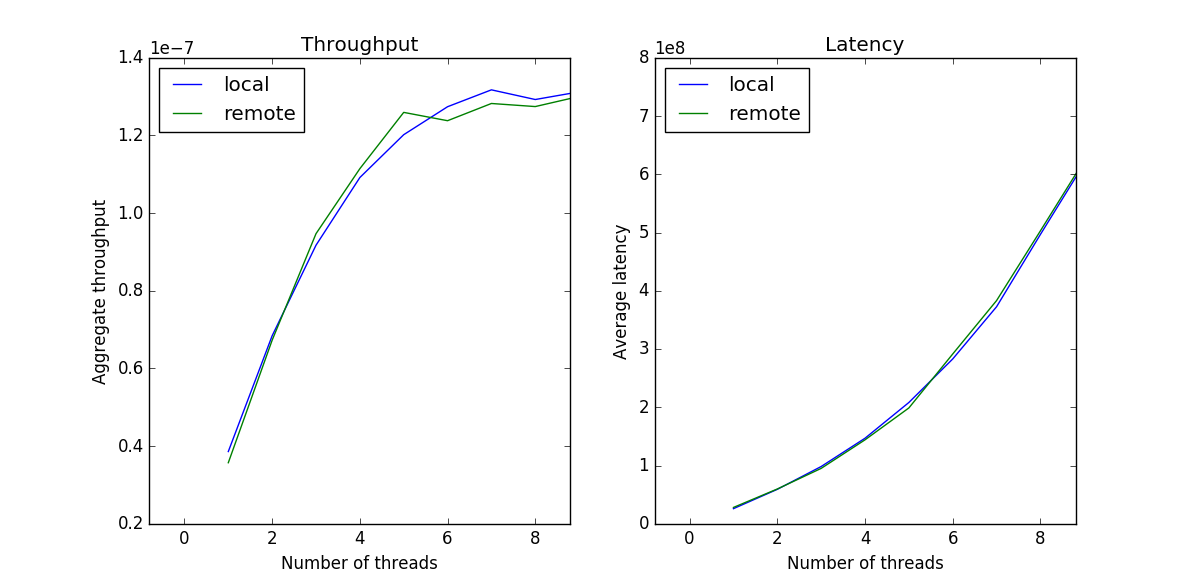
\includegraphics[scale=0.5]{plots.png}
    \label{fig:plots}
    \caption{Plots}
\end{figure}


\subsection{Reliability}
In the interest of profit, from a business perspective, the metric employed
makes sense.

As we increase the number of threads, and hence the performance of the system
being simulated, so does the throughput. Please review the plots above. This
supports that the metric is indeed reliable. In a more rigid way, we argue that
the metric is reliable, as the increase in threads allows for faster and more
frequent restocking that in turn decreases the amount of sales misses, which
means that throughput has increased proportionally with the amount of threads.

We do, however, believe that the metric does not capture some potential
crucial information. And {\it average} or {\it aggregate} projects all
information into a single value that does not capture the overall distribution
of the measured performance. Instead of simply aggregating or averaging the
individual times of the workers, we can construct a histogram of the data and
simply report this instead, as it convey much better data. For instance, we
could answer questions like, are the times normally distributed as one would
perhaps theoretically assume, or are there groups of clients with low and a
group with high latency, whereto the average would tell us little. This way we
can make more solid arguments about the system and its performance overall,
rather than mere successes per time interval. Alternatively. we could report
the suggested metric, as well as minimum, maximum and spread of the latency
and throughput.
